% !TeX document-id = {1082b3d7-4443-4f42-9d9f-82b1b21d1577}

% The BIThesis Template for Graduate Thesis
% Copyright 2020-2023 Yang Yating, BITNP
% Compile with: xelatex -> biber -> xelatex -> xelatex

% !TeX program = xelatex
% !BIB program = biber

% type=master
% type=doctor
% blindPeerReview=true (example: [type=master,blindPeerReview=true])
% twoside=true (example: [type=master,twoside=true])
%

% Under Linux and macOS systems, due to copyright issues, Chinese fonts are different from those under Windows systems.
% If you want to get the same effect as a Word document, you have two options:
% 1. Compile the final paper using Windows system.
% 2. Manually install Zhongyi font and add the option: `\documentclass[...,ctex={fontset=windows}]{bithesis}`.


\documentclass[type=doctor,twoside=false, english=true]{bithesis}

% Only commonly used configurations are listed here. Please see the "bithesis.pdf" manual for all configuration usage.


%%%    !!!!!IMPORTANT!!!!!
%%%%%%%%%%%%%%%%%%%%%%%%%%%%%%%%%%%%%%%%%
%% DONT PLACE ANY BLANK LINE in BITSetup
%%%%%%%%%%%%%%%%%%%%%%%%%%%%%%%%%%%%%%%%%
\BITSetup{
  cover = {
    %% Use this option to change the cover date
    date = 2024年6月,
    autoWidthPadding = 0.25em,
  },
  info = { 	
  	% If you want to delete a certain item of cover information, just delete the item directly.
  	% If you want to leave a certain cover information blank (but keep the underline), please pass in a string composed of whitespace characters, such as "{~}".
  	% If line breaks are required, use "\\" symbols to separate them.
    classification = TQ028.1,
    UDC = 540,
    title = 在虚拟现实中实现非语言互动社交化身的新方法,    
    % To override the vertical title, configure the following options.
    % The following example shows how to use vertical or rotated English in a vertical title.
    % verticalTitle = {形状记忆聚氨酯{L } {T } {X }的合成 \rotatebox[origin=c]{-90}{Feng Kaiyu} 及其在织物中的应用},   
    % verticalTitle = {Title.... {L} {T} {X} \rotatebox[origin=c]{-90}{Feng Kaiyu} and its application},
    titleEn = Novel Methods for Realizing Non-Verbal Interactive Social Avatars in Virtual Reality,
    author =艾力,    
    % If you want to manually control the hidden information in blind review mode, you can use the macro \SecretInfo{}. There are two ways to use it, such as:
    % major = \SecretInfo{Materials Science and Engineering} can get ******* (replace with equivalent substitution symbols)
    % major = \SecretInfo{Materials Science and Engineering}[ABCDEF] can get ABCDEF (replace with your custom content)  
    major = 计算机科学与技术,
    school = 计算机学院,
    degree = 工学硕士,
    chairman = 老师,
    defenseDate = 2024年6月1日,
    supervisor = 老师,
    authorEn = Manjotho Ali Asghar,
    schoolEn = Computer Science,
    supervisorEn = Prof.,
    chairmanEn = Prof. ,
    degreeEn = Doctor of Engineering,
    majorEn = Computer Science and Technology, 
    defenseDateEn = {June, 1st, 2024},
    keywords = {人类运动理解;社交化头像;模糊定性运动学;量化运动令牌。},
    keywordsEn = {Human motion understanding; social avatars; fuzzy qualitative kinematics; quantized motion tokens.}
    % Place in the upper right corner of the cover if necessary and mark in accordance with national regulations.
    % classifiedLevel = confidentiality level\BigStar confidentiality period,
  },
	% Do not display the title of the summary and main symbol comparison table in the contents page.
  TOC = {
    abstract = false,
    abstractEn = false,
    symbols = false,
  },
  style = {
    pageVerticalAlign = scattered,
    % Enable Zhongyi Song font pseudo-bold font under Windows platform.
    % windowsSimSunFakeBold = true,
  },
  publications = {
    % The following two options will affect the omission threshold of the name list in the "List of Papers and Research Results Published During the Degree Study".
    % Generally speaking, if you are ranked fourth lowest among all documents, it is recommended that you set both values ​​to 4.
    % See the manual for more detailed instructions.
    maxbibnames = 3,
    minbibnames = 1,
  },
  % Adopt chapter title level appendix format
  appendices / chapterLevel = true,
  const = {
    % Due to the inconsistency between the existing Word template and the old LaTeX template and the "Beijing Institute of Technology Graduate Thesis Writing Standards",
    % Some fields on the paper cover require users to manually adjust them according to their own circumstances.
    % The default value currently given is set in accordance with the requirements in the "Guidelines for Writing Postgraduate Dissertations of Beijing Institute of Technology" released in 2018.
    % For example, the commented out line will change the "Application for Degree Level" in the cover page to "Application for Degree".
    % info / degree = {Apply\quad{}please\quad{}study\quad{}degree},
    % info / major = {study\quad{}subject\hspace{5pt}/\hspace{5pt}category\quad{}category}
  }
}

% Most modifications to the reference style can be configured through the options here.
% Please search "biblatex-gb7714-2015 document" for details.
\usepackage[
  defernumbers=true,
  backend=biber,
  style=gb7714-2015,
  gbalign=gb7714-2015,
  gbnamefmt=lowercase,
  gbpub=false,
  gbannote=true,
  gbpunctin=false,
  doi=false,
  url=false,
  eprint=false,
  isbn=false,
]{biblatex}


% Add references
\addbibresource{reference/main.bib}
% List of papers and research results published during the degree study. For detailed usage, please see `chapters/pub.tex`.
\addbibresource{reference/pub.bib}


\usepackage{graphicx}
\usepackage{makecell}
\usepackage{booktabs}
\usepackage{algorithm}
\usepackage{algorithmicx}
\usepackage{algpseudocode}
\usepackage{rotating}
%\usepackage{setspace}

\begin{document}

% Print title page
\MakeCover


% Print spine
\MakePaperBack

% Chinese information and English information
\MakeTitle

% Paper originality statement and use authorization
\MakeOriginality

%%%%%%%%%%%%%%%%%%%%%%%%%%%%%%
%% Prefix
%%%%%%%%%%%%%%%%%%%%%%%%%%%%%%
\frontmatter

% Abstract
%%
% The BIThesis Template for Graduate Thesis
%
% Copyright 2020-2023 Yang Yating, BITNP
%
% This work may be distributed and/or modified under the
% conditions of the LaTeX Project Public License, either version 1.3
% of this license or (at your option) any later version.
% The latest version of this license is in
%   http://www.latex-project.org/lppl.txt
% and version 1.3 or later is part of all distributions of LaTeX
% version 2005/12/01 or later.
%
% This work has the LPPL maintenance status `maintained'.
%
% The Current Maintainer of this work is Feng Kaiyu.



%The abstract is an independent and complete short article that should summarize and succinctly reflect the main content of the paper. Including research purpose, research methods, research results and conclusions, etc., especially highlighting the research results and conclusions. The Chinese abstract strives to be concise and accurate in language. The recommended length for a doctoral thesis is 1000-1200 words, and the recommended length for a master's thesis abstract is 500-800 words. References, figures, tables, chemical structural formulas, non-publicly known symbols and terms are not allowed to appear in the abstract. The content of the English abstract and the Chinese abstract should be completely consistent, the grammar and wording should be accurate, and the language should be concise and smooth. The English version of the doctoral dissertation of international students should have a "detailed Chinese abstract" of no less than 3,000 words.)

\begin{abstract}
人类运动的理解在各个领域都至关重要,包括计算机图形学、机器人技术、医疗保健和交互式模拟。然而,传统方法通常难以有效地弥合动作语义和行为理解之间的差距,这是由于表示不足和运动层次结构中固有的不确定性所导致的。本论文提出了创新性的解决方案,以增强对人类运动的理解和生成。

首先,我们深入研究了人类运动理解的复杂性,并引入了一种称为模糊定性运动学(FQK)的新方法。这一开创性的框架将模糊推理和定性推理相结合,以便于对富有表现力和不确定性的运动事实进行建模。通过为各种运动属性创建模糊语言变量、术语和隶属函数,FQK实现了从运动序列中提...
\end{abstract}

\begin{abstractEn}
Understanding human motion is crucial in various fields, including computer graphics, robotics, healthcare, and interactive simulations. However, traditional methods often struggle to effectively bridge the gap between motion semantics and action comprehension due to inadequacies in representations and inherent uncertainties in kinematic hierarchies. This thesis proposes innovative solutions for enhancing the understanding and generation of human motion.

First, we delve into the complexities of human motion comprehension and introduce a novel approach termed Fuzzy Qualitative Kinematics (FQK). This groundbreaking framework combines fuzzy inference and qualitative ...
\end{abstractEn}


% Table of contents
\MakeTOC

% List of figures
\listoffigures

% List of tables
\listoftables

% Symbol table
%%
% The BIThesis Template for Graduate Thesis
%
% Copyright 2020-2023 Yang Yating, BITNP
%
% This work may be distributed and/or modified under the
% conditions of the LaTeX Project Public License, either version 1.3
% of this license or (at your option) any later version.
% The latest version of this license is in
%   http://www.latex-project.org/lppl.txt
% and version 1.3 or later is part of all distributions of LaTeX
% version 2005/12/01 or later.
%
% This work has the LPPL maintenance status `maintained'.
%
% The Current Maintainer of this work is Feng Kaiyu.

\begin{symbols}
  \item[BIT] 北京理工大学的英文缩写
  \item[\LaTeX] 一个很棒的排版系统
  \item[\LaTeXe] 一个很棒的排版系统的最新稳定版
  \item[ctex] 成套的中文\LaTeX{}解决方案,由一帮天才们开发
  \item[$ e^{\pi{}i}+1=0$] 一个集自然界五大常数一体的炫酷方程
\end{symbols}


\mainmatter

% Please add chapters in order according to the content of the paper.

\chapter{Introduction}

\section{Background}
Human motion generation using skeleton-based 3D motion data has gained significant attention from researchers across various fields, including computer graphics, robotics, human-computer interaction (HCI), and computer vision. The primary objective of human motion generation is to develop models that are capable of synthesizing realistic, natural, and diverse human motions. These synthesized motions find applications across a broad spectrum, including digital film production, games, augmented/virtual reality (AR/VR), sports analysis, smart healthcare, human-robot interaction (HRI), and the creation of intelligent virtual avatars (IVAs).

Typically, a human motion generation task is conditioned on various factors, such as text \cite{dummy}, audio \cite{dummy}, scene \cite{dummy}, or another motion sequence \cite{dummy}. In recent years, there has been a significant surge in the development of diverse generative methods, primarily driven by advancements in deep learning \cite{dummy}. These approaches include Autoregressive models \cite{dummy}, Variational Autoencoders (VAE) \cite{dummy}, Normalizing Flows \cite{dummy}, Generative Adversarial Networks (GAN) \cite{dummy}, and Denoising Diffusion Probabilistic Models (DDPM) \cite{dummy}. These methodologies have demonstrated their effectiveness in various domains such as text \cite{dummy}, \cite{dummy}, imagery \cite{dummy}, video \cite{dummy}, and 3D objects \cite{dummy}. Additionally, significant progress in human motion modelling \cite{dummy} has enabled the extraction of human motion from videos \cite{dummy}, as well as the creation of extensive human motion datasets \cite{dummy}. Consequently, there has been growing interest within the research community in data-driven approaches for human motion generation in recent times.

Human motion generation presents several challenges ...


\begin{figure}[t]	
	\centering
	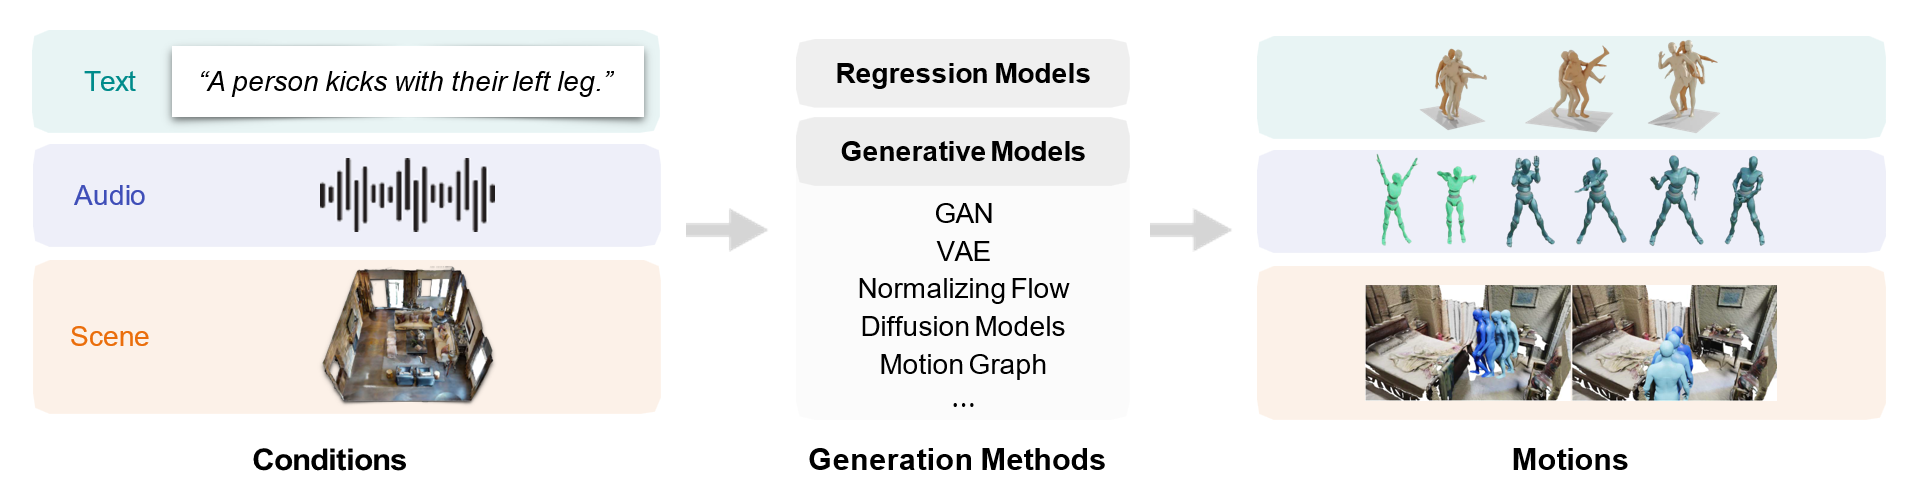
\includegraphics[width=1\textwidth]{figures/chapter1/fig_hmg_gan}
	\caption{An overview of typical human motion generation approaches. Example images adapted from \cite{dummy}.}
	\label{fig_hmg_gan}
\end{figure}
 
\section{Motivation}
Generating accurate 3D motions is a hot topic in the field of computer vision. Researchers are proposing various methods to generate human motions, such as predicting motions based on historical sequences, generating motions for a particular action class, and creating motions that follow a trajectory or a song. These methods aim to produce increasingly realistic and complex motions. There are numerous potential applications for these generative methods in various areas, which has sparked the interest of researchers.\\

\subsection{Human-Robot Interaction (HRI)}

\noindent
Safe and Efficient Collaboration: The utilization of human motion generation in training robots to predict human movements results in enhanced collaboration efficiency and safety within shared work environments. The simulation of various human actions enables robots to adapt their behavior and movements accordingly, thereby reducing the occurrence of collisions or accidents.

\noindent
Enhanced Robot Configuration: Through the generation of diverse and intricate human motions, scholars can assess and enhance the design of robots. This process involves examining a robot's capacity to maneuver ...


\section{Research Gaps in Existing Studies}
Despite the progress made in human motion generation, there exist significant gaps and opportunities for further research and development. We identify the following limitations and lack of research in the domain:\\

\noindent
\textbf{Bridging action semantics and raw motion}: The fundamental challenge lies in establishing a meaningful connection between the raw motion space and the action semantic space \cite{dummy}. Conventionally, raw motion is represented as a sequence of 3D poses \cite{dummy} or SMPL model parameters \cite{dummy}, while action semantics are characterized by action categories or textual descriptions in natural language. Existing approaches for human motion generation often struggle to produce realistic motion sequences due to significant gap in mapping from action semantic text to raw motion pose sequence. Creating stronger connection between action semantics and raw motion with the aid of intermediate motion representations can make human motion understand more intuitive and improve the performance of underlying motion tasks. \\

\noindent
\textbf{Human reaction motion generation}: Existing research mostly focus on generating human motion for a single character, while neglecting the motion sequences where interaction of two persons are involved. There is an opportunity for creating methods that generate reactive motion of one character when the action sequence of other is given.\\

\noindent
\textbf{Human interaction generation}: Existing methods recognize and label the human interactions, but there is a lack of research pertaining to generation of motion sequences for interacting characters.\\

\noindent
\textbf{Accurate 3D human pose estimation}: In human-agent interactions, 3D human pose estimation is fundamental. The quality of extracted 3D skeletons for human motion is directly proportional to the accuracy of motion models. Despite recent progress in 3D human pose estimation methods, practical applications often encounter challenges, particularly when dealing with complex poses commonly found in human motion sequences. Proposing an accurate 3DHPE method dealing with complex poses can benefit more accurate human motion generation models.



\begin{figure}[!t]	
	\centering
	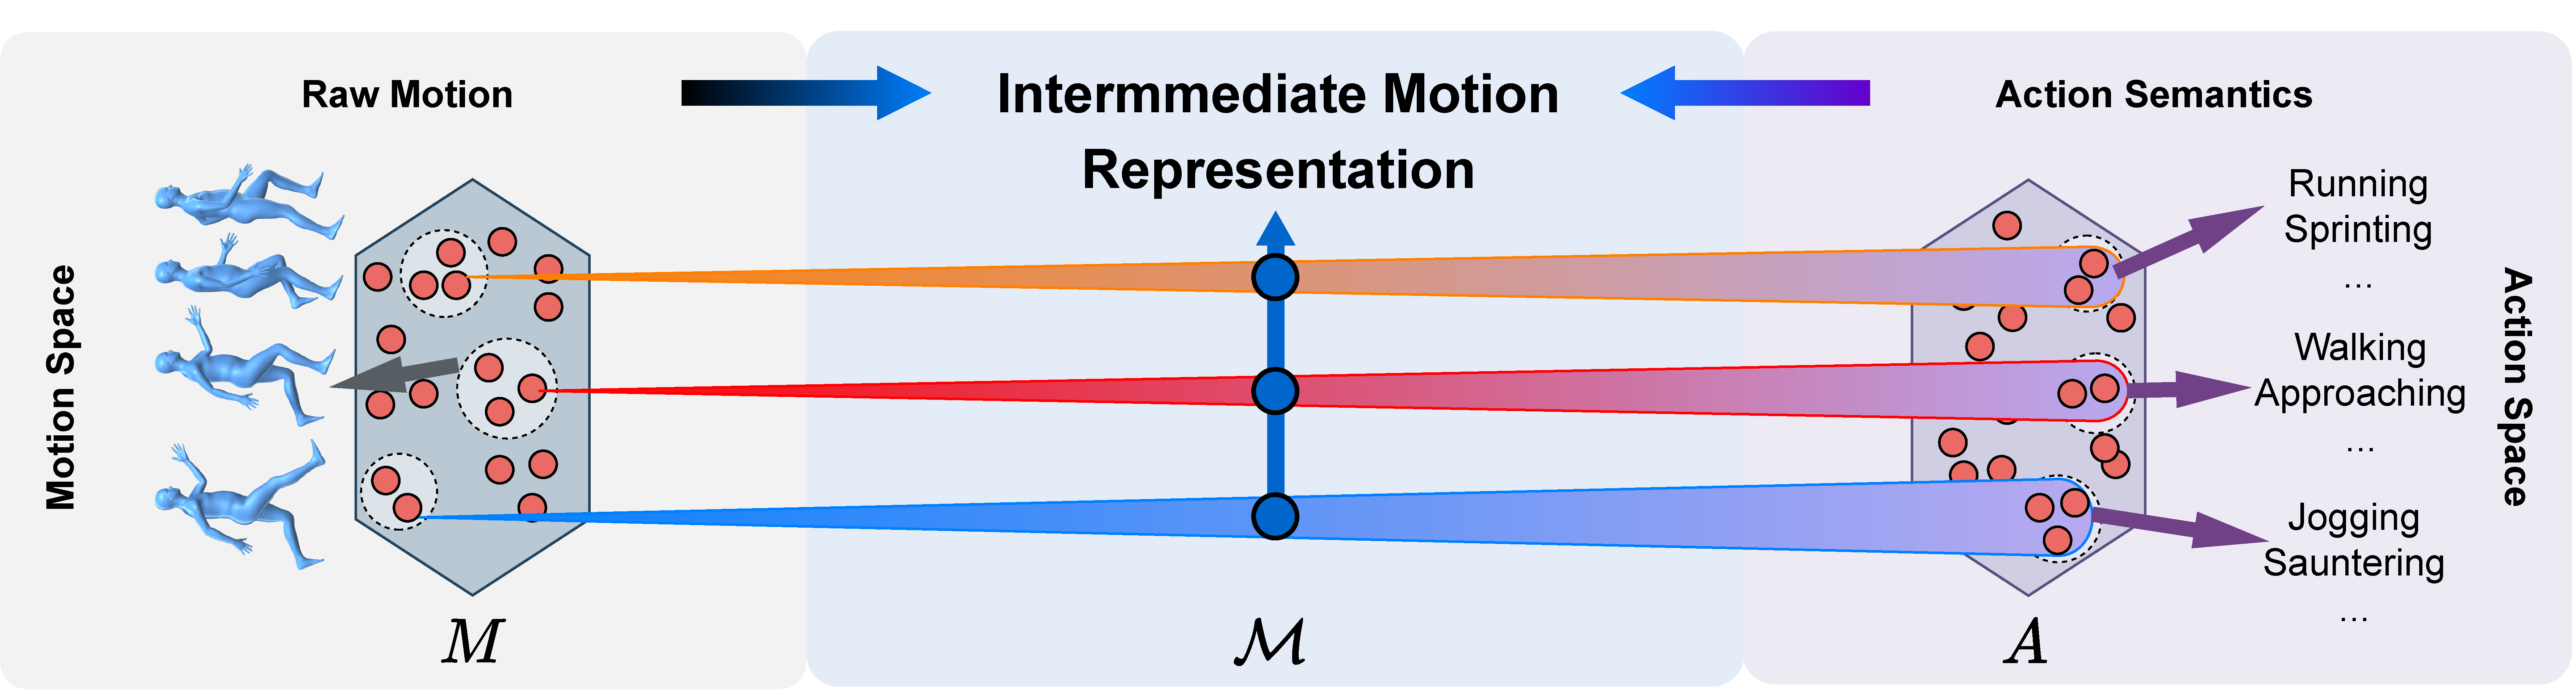
\includegraphics[width=1\textwidth]{figures/chapter1/fig_problem_statement_1}
	\caption{Visualizing semantic gap between action semantics and raw motion.}
	\label{fig_problem_statement_1}
\end{figure}

\begin{figure}[!t]	
	\centering
	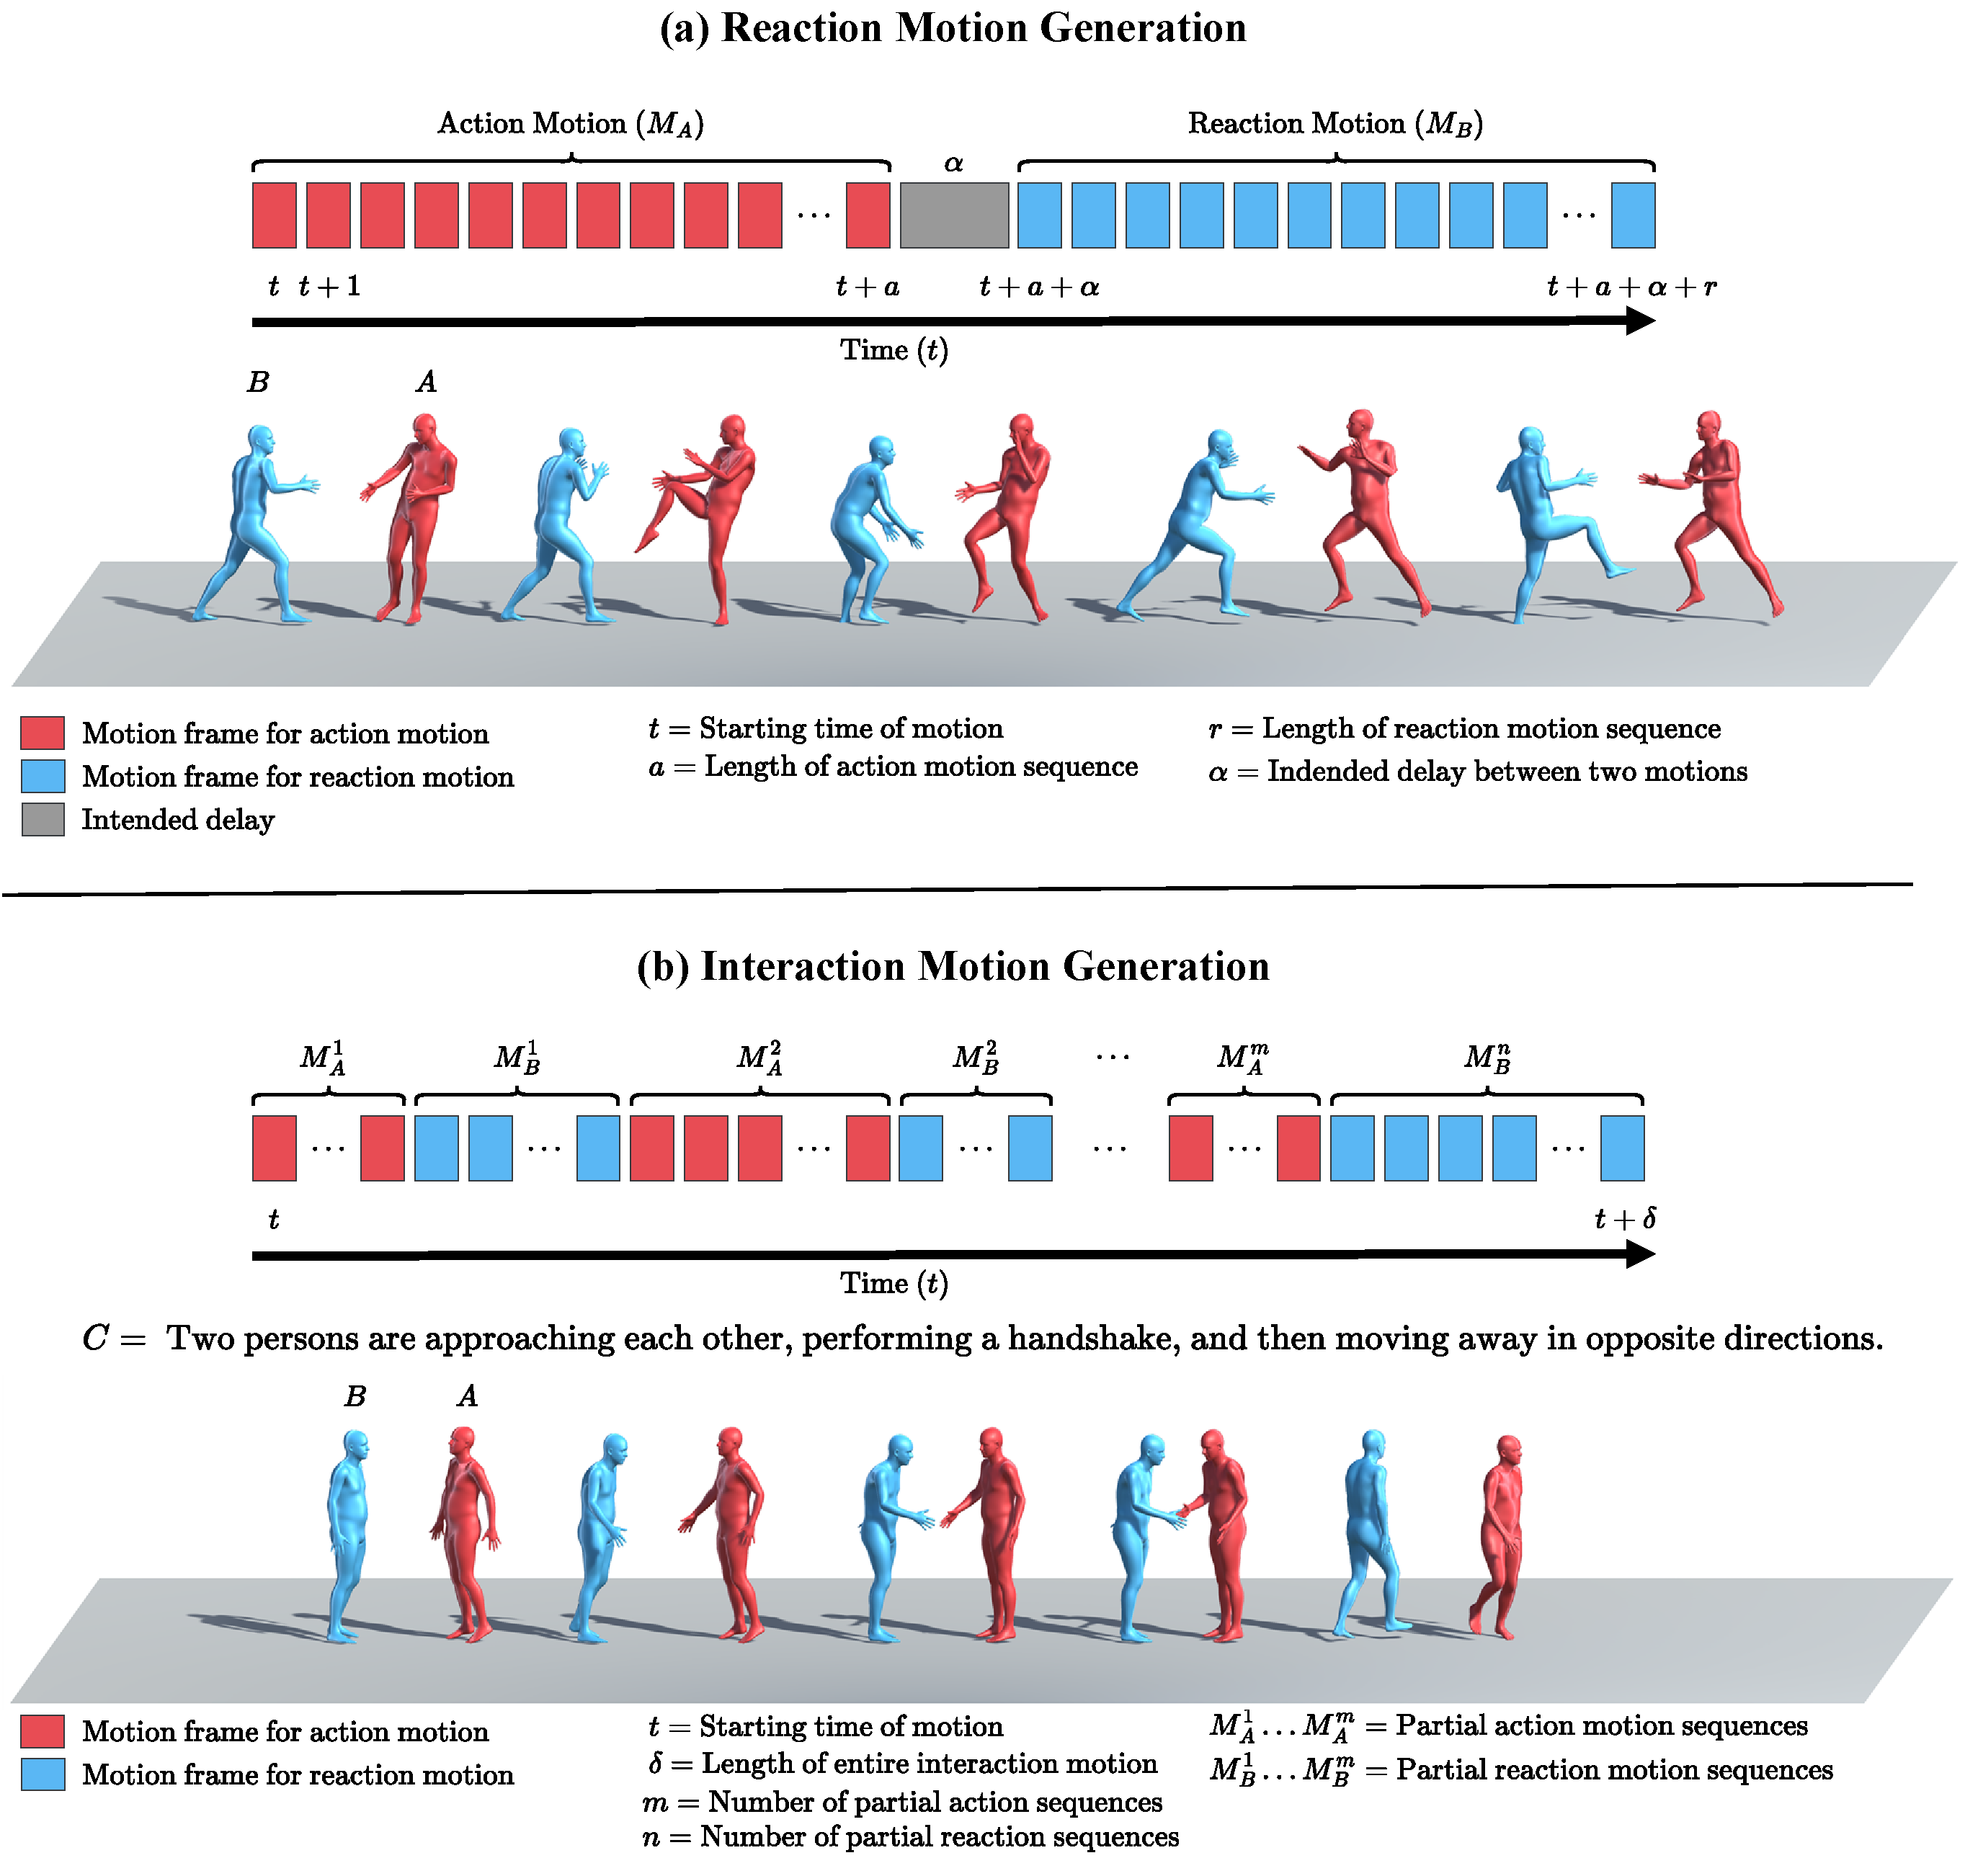
\includegraphics[width=1\textwidth]{figures/chapter1/fig_problem_statement}
	\caption{Illustration and mathematical symbols for various human motion generation process. The virtual character in red (Character A) represents the actor performing an action sequence. The character in blue (Character B) represents the actor performing a reaction sequence. (a) The illustration for reaction generation, when action motion sequence is given. (b) The illustration for interaction generation, given the conditioned signal $C$.}
	\label{fig_problem_statement}
\end{figure}




\section{Problem Formulation}
Consider the reaction motion generation concept illustrated in Fig.\ref{fig_problem_statement} (a) and interaction motion generation shown in Fig. \ref{fig_problem_statement} (b), we define following problem statements for this thesis:

\begin{enumerate}
	\item Developing an effective methodology to bridge action semantics $A$ and raw motion $M$ by generating an stronger intermediate motion representation $\mathcal{M}$. The intermediate representation is devised such that the mapping $A\mapsto \mathcal{M} \mapsto M$, ultimately leads to motion generation characterized by improved precision, diversity, multi-modality, and accuracy across various motion generation tasks.
	\item Given a action motion sequence $M_B$ of virtual character $B$, develop a motion generator network to generate corresponding reaction motion sequence $M_A$ of character $A$, where $M_A \in \mathbb{R}^{T \times J \times 3}$ and $M_B \in \mathbb{R}^{T \times J \times 3}$ are the sequences of skeleton poses with $J$ number of joints and $T$ number of frames.
	\item Developing a motion generation network to simultaneously generate partial interactive motion sequences ${M_A^1, \dots, M_A^m}$ and ${M_B^1, \dots, M_B^n}$ for character $A$ and character $B$, respectively, given a textual context $C$ in a dyadic interaction scenario. Where each partial motion $M_A^M \in \mathbb{R}^{T \times J \times 3}$ and $M_B^N \in \mathbb{R}^{T \times J \times 3}$ are the sequences of skeleton poses with $J$ number of joints and $T$ number of frames (while $T$ may be variable for each sequence).
	\item Given a monocular RGB image $I$, develop an pose estimation network to output a 3D human pose $P$, where $P \in \mathbb{R}^{J \times 3}$ and $J$ is the number of skeleton joints.
\end{enumerate}


\section{Research Questions}

The study identifies and tries to answer the following research questions:

RQ1: How can intermediate motion representations effectively bridge the gap between action semantics and raw motion, improving the realism of generated motion sequences?

RQ2: What novel methods can be devised to generate reactive motion sequences for a character in response to the action sequence of another character?

RQ3: How can motion generation networks be designed and trained to accurately produce motion sequences for interacting characters in dyadic interactions?

RQ4: What advancements can be made in 3D human pose estimation to enhance the accuracy of extracted poses, particularly in dealing with complex poses commonly found in human motion sequences?

RQ5: How can a comprehensive framework integrating improved pose estimation, action-motion semantic comprehension, reaction motion modeling, and interactive motion modeling be designed and implemented to improve the naturalness and realism of generated human motion sequences?


\section{Research Aim and Objectives}
This aim of the study is to proposes a comprehensive framework to facilitate the generation of human motion sequences, incorporating coarse-to-fine pose estimation, action semantic comprehension, reaction motion modeling, and interactive motion modeling to improve the realism and naturalness of the generated motion sequences. The objective of the study are:

\begin{enumerate}
	\item To identify and propose intermediate motion representation to effectively bridge action semantics and raw motion.
	\item Designing and developing a network to generate the reaction motion sequence given the action motion sequence.
	\item Designing and developing a network to generate interaction motion sequence in dyadic interactions.
	\item Designing and developing an accurate 3D human pose estimation network to yield a 3D human pose given a monocular image. 
\end{enumerate}


\section{Significance of the study}
This research holds significant implications for numerous applications, including entertainment, education, healthcare, and human-computer ...



\section{Contributions of the Study}
This thesis makes several contributions to the field of human motion synthesis, including novel algorithms, methodologies, and insights that address key challenges and advance the state-of-the-art...

\section{Thesis Organization}
\noindent
Chapter 2: This chapter provides a comprehensive ...

\noindent
Chapter 3: This chapter introduces a novel methodology ...

\noindent
Chapter 4: This chapter presents a novel approach ...

\noindent
Chapter 5: This chapter employs anthropometric constraints ...



\begin{figure*}[!t]
	\centering
	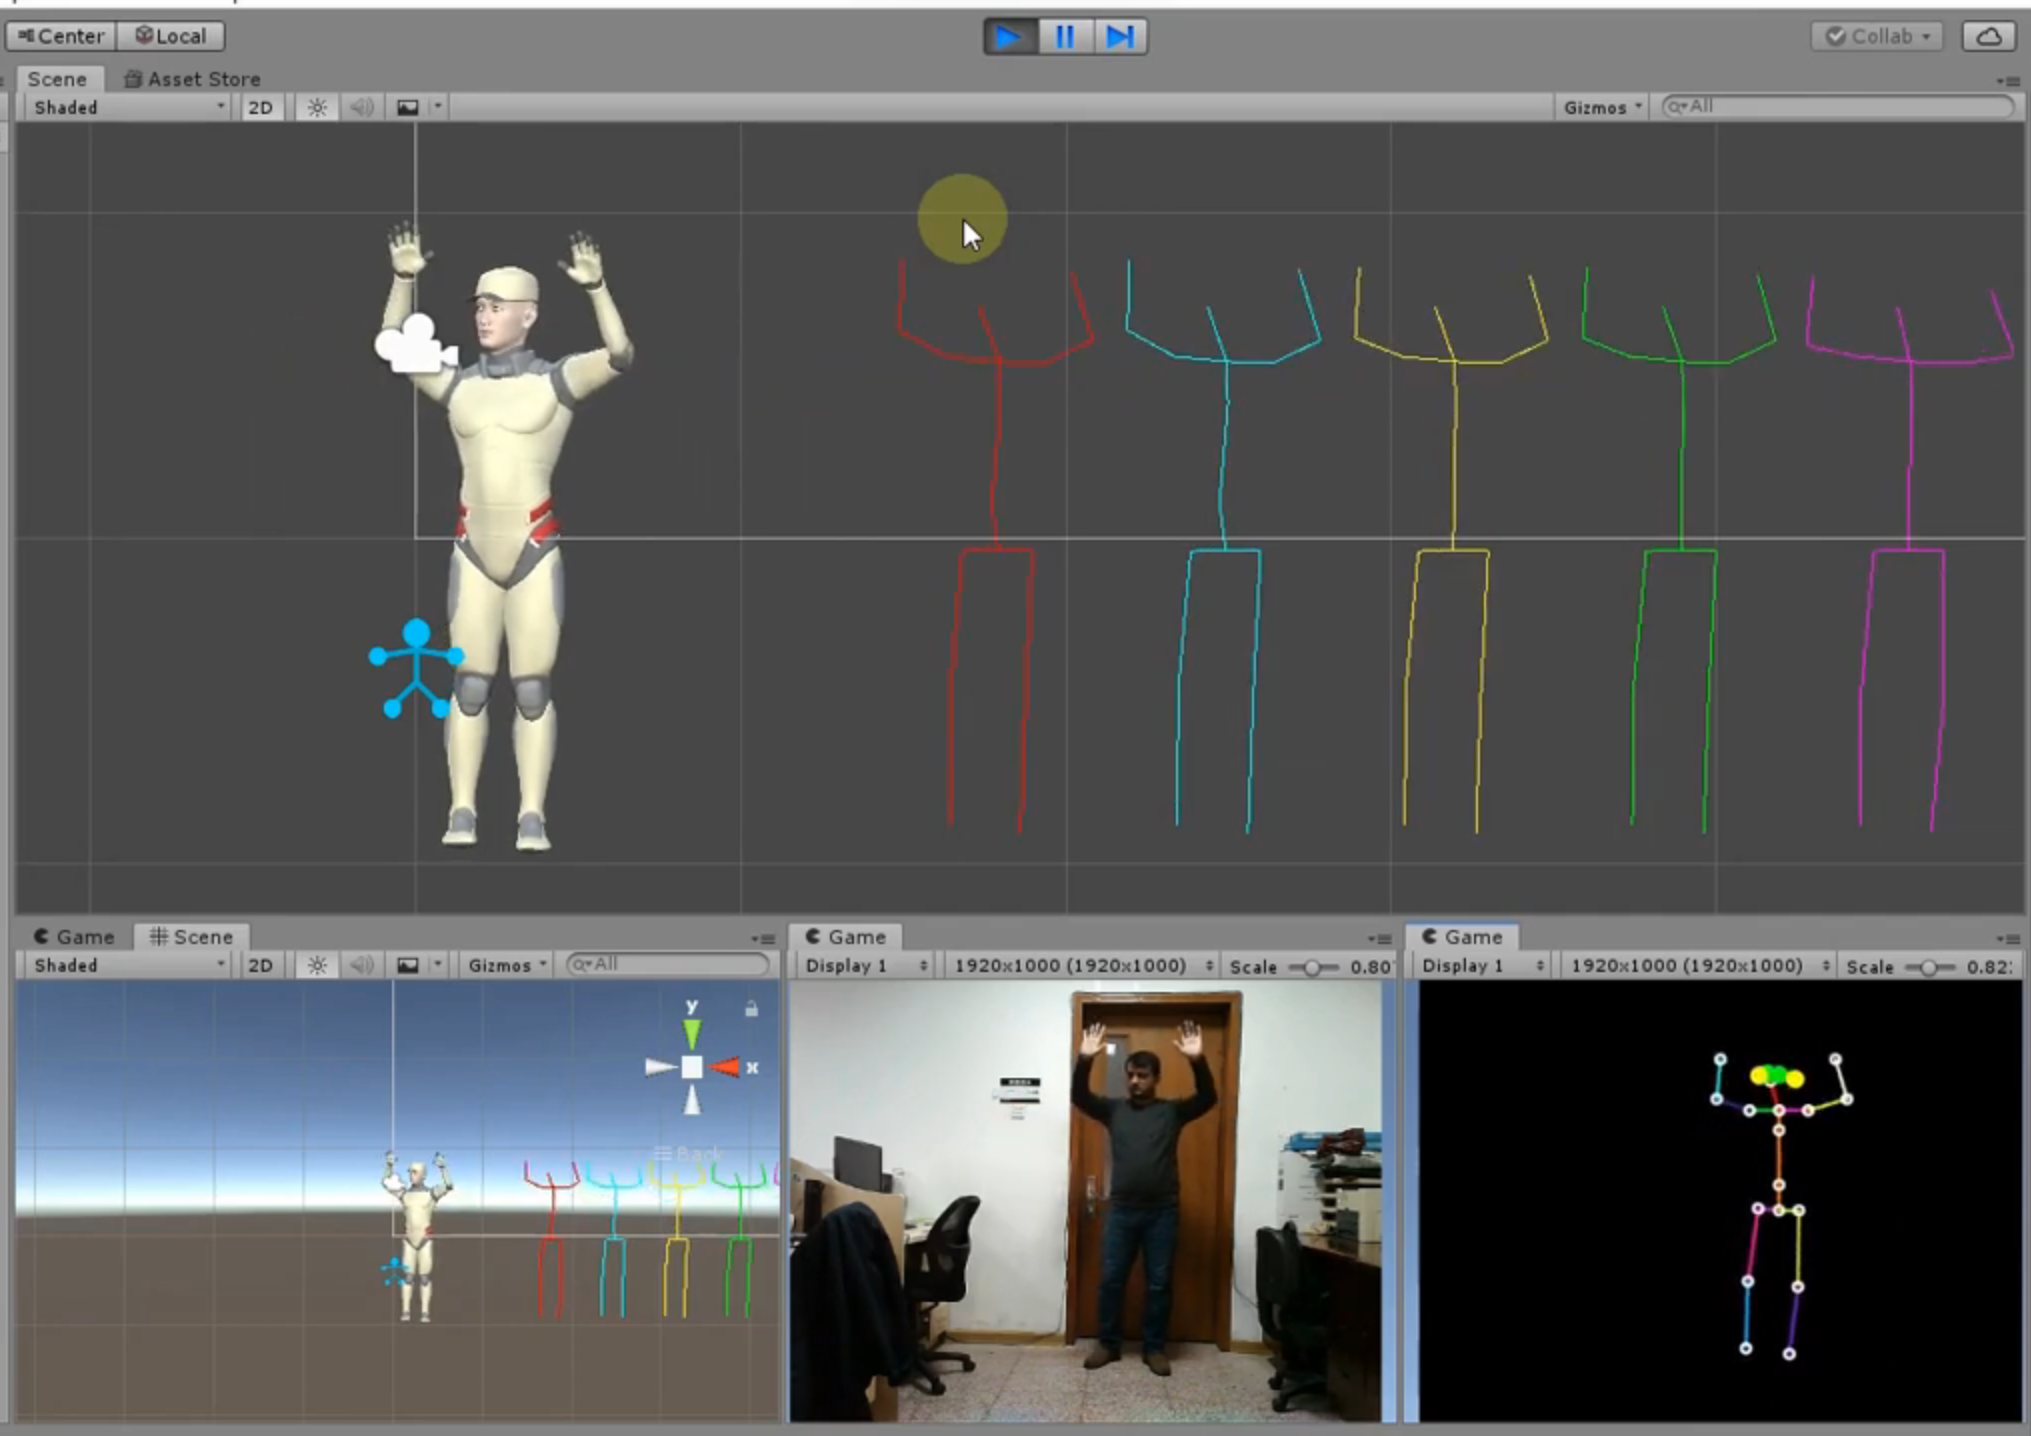
\includegraphics[width=1\textwidth]{figures/chapter1/fig_human_avatar_2}
	\caption{Human avatar interaction in virtual reality.}
	\label{fig_gap}
\end{figure*}





%%
% The BIThesis Template for Graduate Thesis
%
% Copyright 2020-2023 Yang Yating, BITNP
%
% This work may be distributed and/or modified under the
% conditions of the LaTeX Project Public License, either version 1.3
% of this license or (at your option) any later version.
% The latest version of this license is in
%   http://www.latex-project.org/lppl.txt
% and version 1.3 or later is part of all distributions of LaTeX
% version 2005/12/01 or later.
%
% This work has the LPPL maintenance status `maintained'.
%
% The Current Maintainer of this work is Feng Kaiyu.
%
% Compile with: xelatex -> biber -> xelatex -> xelatex

\chapter{Literature Review}

Human beings exhibit a remarkable ability to plan and execute body movements in response to their intentions and environmental stimuli \cite{dummy}. This intrinsic capability has become a central pursuit within artificial intelligence research, as there is a growing interest in the development of algorithms capable of generating motion patterns that mimic human behavior. This interdisciplinary endeavor has attracted attention from a myriad of research domains, such as computer vision \cite{dummy}, computer graphics \cite{dummy}, multimedia \cite{dummy}, robotics \cite{dummy}, and human-computer interaction \cite{dummy}. The objective of human motion generation is to create natural, lifelike, and diverse human motions, which hold immense potential for application across various fields including film production, video games, augmented and virtual reality (AR/VR), human-robot interaction, and digital human representation.

\section{Motion Data Representation}
Human motion data is effectively represented by sequences of human body poses across the temporal ...

\subsection{Keypoint-based Representation}
In keypoint-based representation, the human body is depicted through a series of keypoints, denoting specific anatomical...

\subsection{Rotation-based Representation}
Another prevalent method for representing human pose involves joint angles, signifying the rotation of body parts or segments ...



\subsection{The SMPL Model}
The Skinned Multi-Person Linear (SMPL) model is parameterized by a set of pose and shape parameters, facilitating the generation of a 3D mesh representing a human body in a specific pose and shape (as illustrated in Figure \ref{fig_1})...





%%
% The BIThesis Template for Graduate Thesis
%
% Copyright 2020-2023 Yang Yating, BITNP
%
% This work may be distributed and/or modified under the
% conditions of the LaTeX Project Public License, either version 1.3
% of this license or (at your option) any later version.
% The latest version of this license is in
%   http://www.latex-project.org/lppl.txt
% and version 1.3 or later is part of all distributions of LaTeX
% version 2005/12/01 or later.
%
% This work has the LPPL maintenance status `maintained'.
%
% The Current Maintainer of this work is Feng Kaiyu.
%
% Compile with: xelatex -> biber -> xelatex -> xelatex

\chapter{Connecting Action Semantics and Human Motion using Fuzzy Qualitative Kinematics}

Human motion understanding is fundamental to various applications in computer graphics, human-robot interactions, digital environments, and entertainment. Existing approaches predominantly rely on modeling motion with quantitative or qualitative kinematic facts. However, they often struggle to establish a robust connection between motion and corresponding action semantics...

\section{Introduction}
Human motion understanding is integral to numerous applications, including human-robot interaction, automated computer animations, social humanoid in augmented/virtual reality, intelligent non-playing characters (NPCs) in video games, physical fitness, sport analysis, and digital film production \cite{fg-t2m, act-recog, assist-walk}. The fundamental challenge lies in establishing a meaningful connection between the raw motion space and action semantic space ...
.

\section{Related Work}
\subsection{Human Motion Representation} 
An accurate representation of human motion is critical for generating realistic motion sequences \cite{motion-synthesis-survey}. Conventional motion is typically represented as a sequence of static pose representations characterized by joint...

\begin{figure*}[!t]
	\centering
	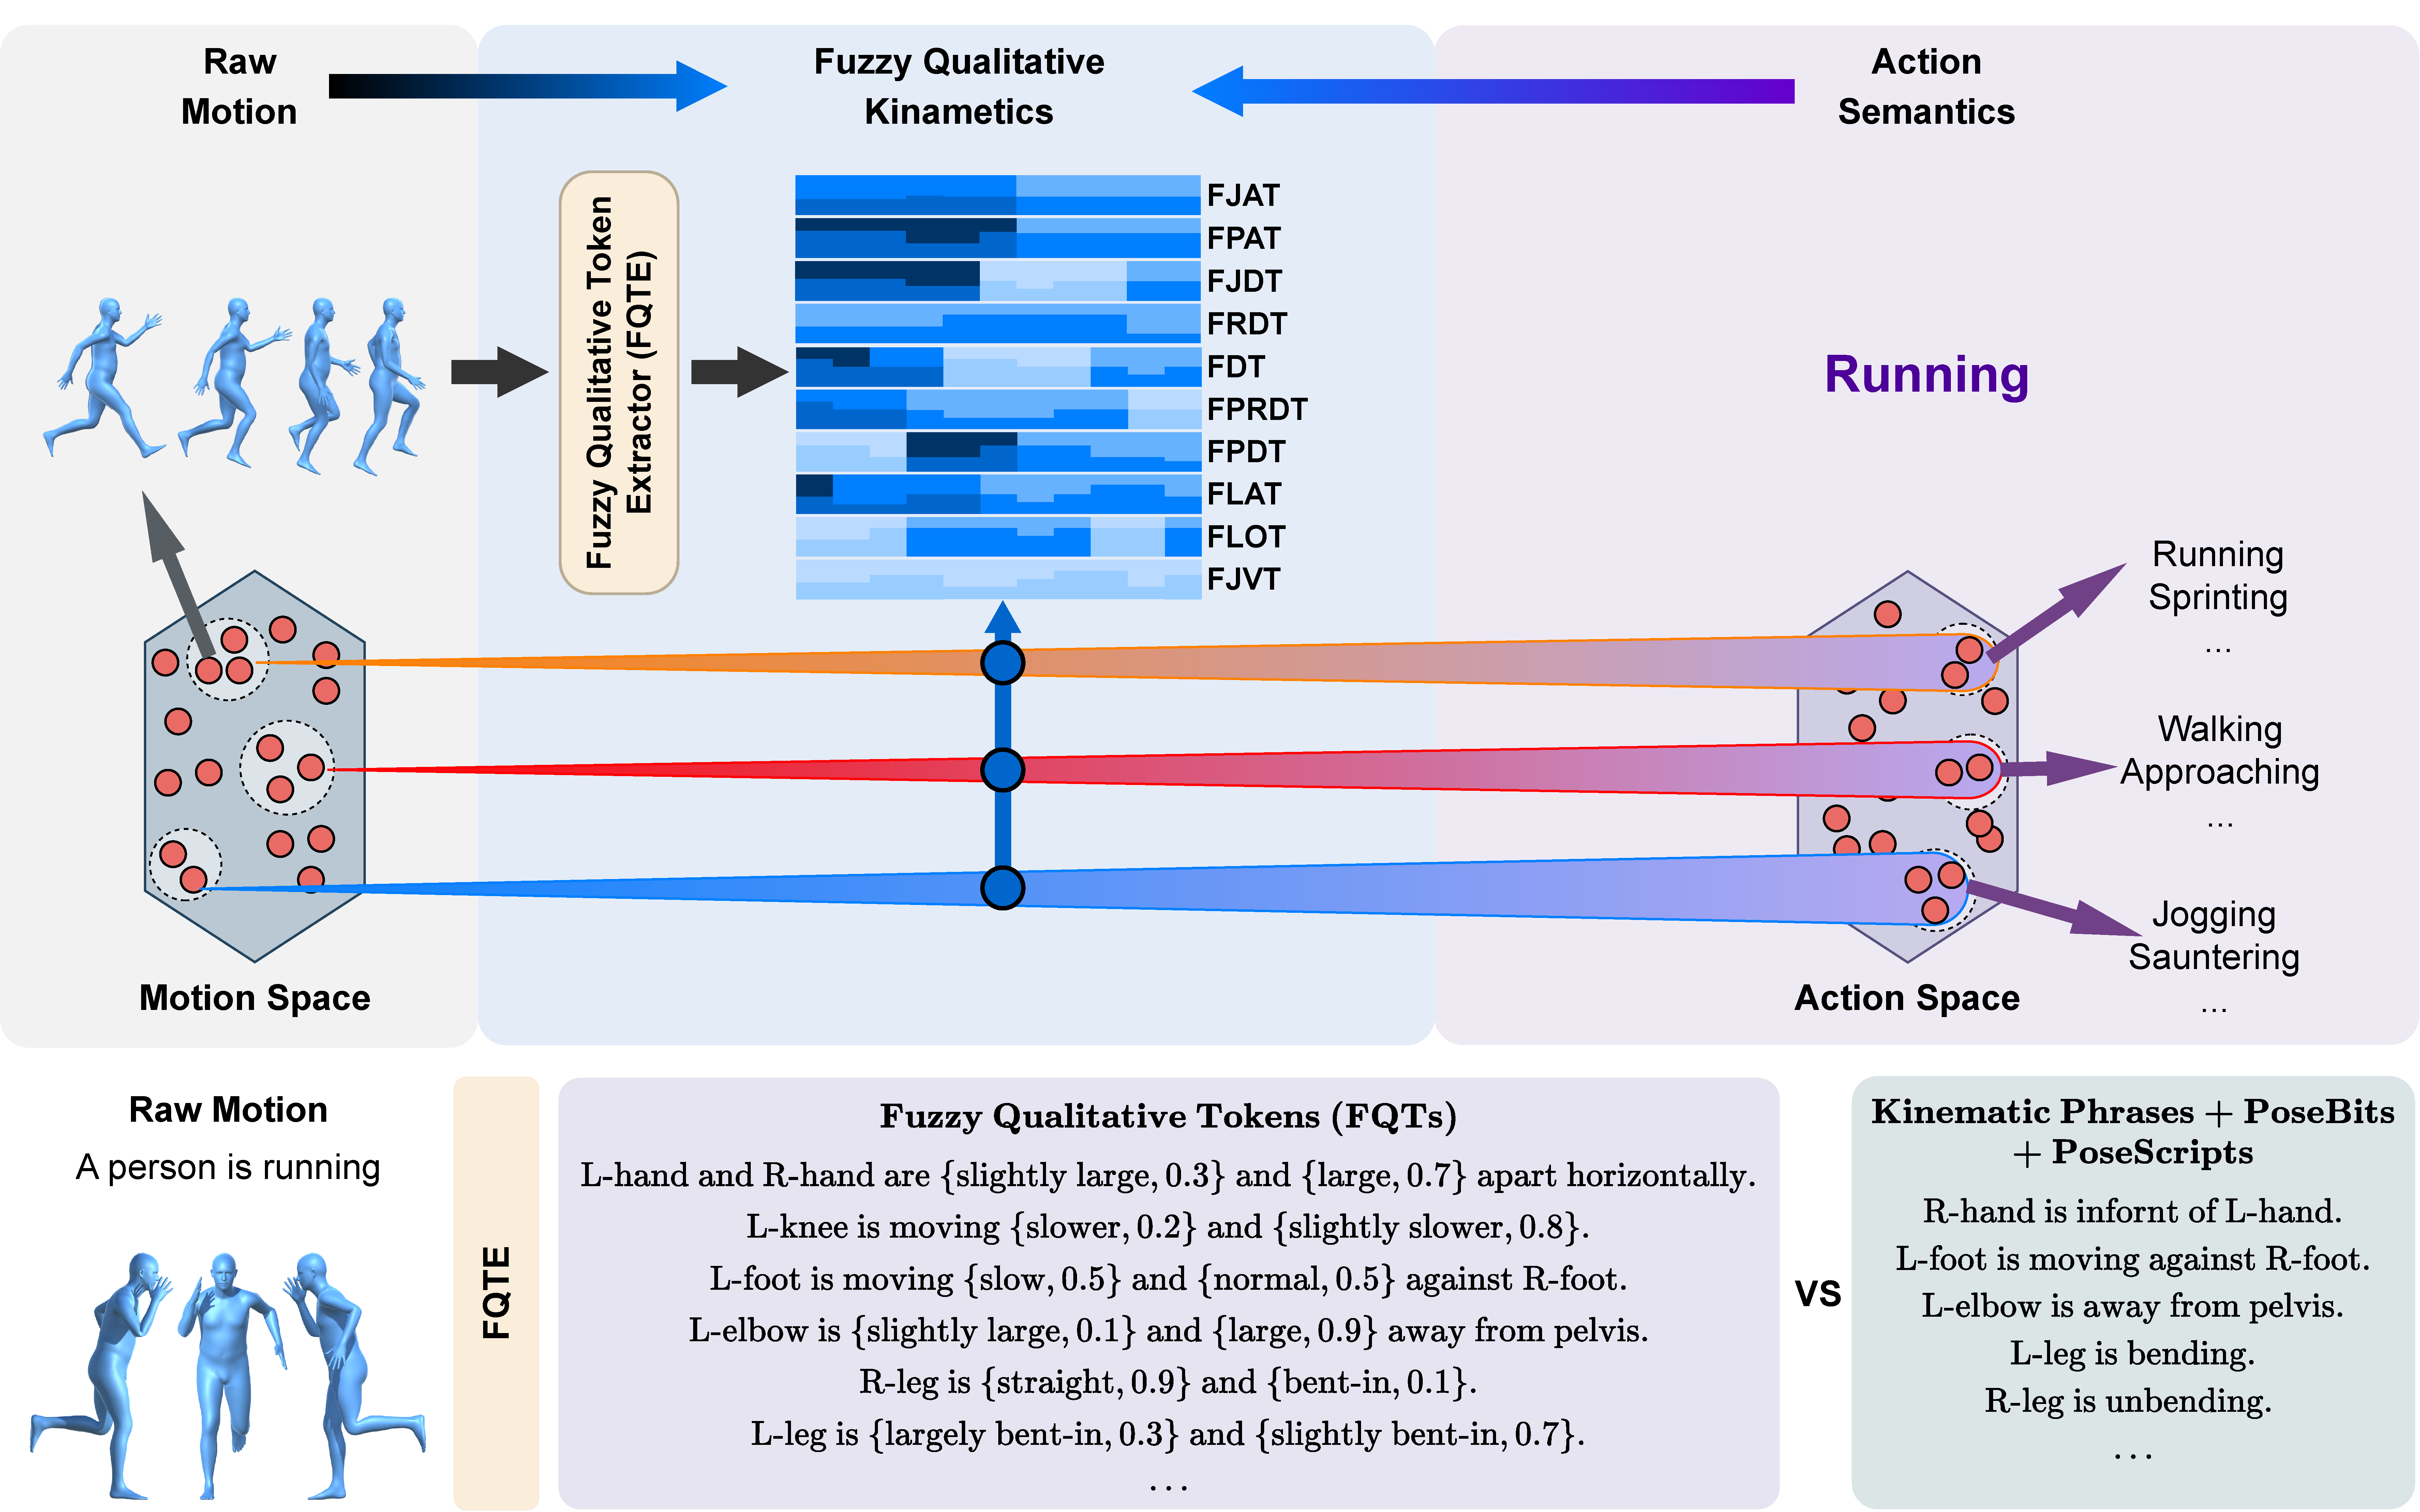
\includegraphics[width=1\textwidth]{figures/chapter3/fig_semantic_gap}
	\caption{(Top) Illustrates the gap between two motion modalities, i.e., raw motion and action descriptions. Understanding human motion requires modeling a complex many-to-many mapping function between motion and action spaces. Fuzzy Qualitative Tokens (FQTs) are presented as an intermediate representation to bridge the gap (bottom) comparison of boolean kinematic facts used by previous studies \cite{kinematic-phrases, pose_bits, pose_script} with our FQTs. FQTs provide expressive pose geometry and rich semantic information.}
	\label{fig_gap}
\end{figure*}




\section{Method}
\noindent
Effective mapping between the action and motion spaces is key to the success of any task involving motion. Fig. \ref{fig_gap} visually demonstrates the semantic gap between these two ...

\subsection{Quantized Fuzzy Membership Function}
\noindent
The standard fuzzy membership function assigns membership scores to crisp input values. However, the conventional real-value membership scale is computationally expensive. To address this issue, we introduce a quantized fuzzy membership function that strikes a balance between representational accuracy and computational complexity, as shown in Fig. \ref{fig_fuzzy}. This quantized fuzzy function extends the standard membership function by translating the real-valued membership scale into a quantized scale. The standard and quantized membership functions represented by the four-tuple $\left[ a, b, c, d \right] $ are defined by eq \eqref{eq_smem} and \eqref{eq_qmem}, respectively.
\begin{equation}
	\label{eq_smem}
	\mu(x) = 	
	\begin{cases}
		0 & \text{if } x \leq a \\
		(x-a)/(b-a), & \text{if } a \leq x \leq b \\
		1, & \text{if } b \leq x \leq c \\
		(d-x)/(d-c), & \text{if } c \leq x \leq d \\
		0, & \text{if } d \leq x
	\end{cases}
\end{equation}
\begin{equation}
	\label{eq_qmem}
	\dot{\mu}(x) = \lfloor \mu(x) \times \mu_{ql} \rfloor /\mu_{ql}
\end{equation}

Where $\mu(.)$ and $\dot{\mu}(.)$ are the standard and quantized membership functions, respectively. The $x$ denotes the crisp value, with $\mu_{ql}$ referring to the number of quantization levels. 



\begin{figure}
	\centering
	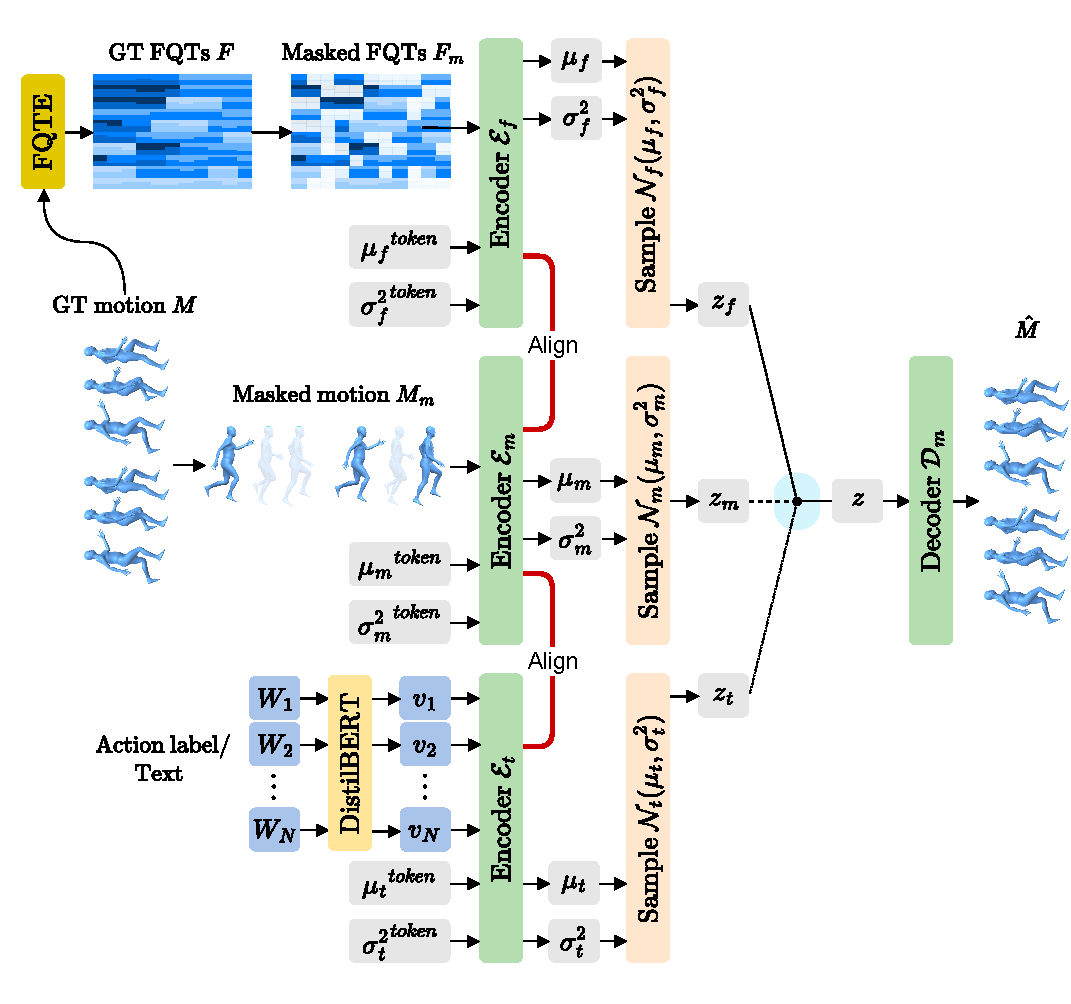
\includegraphics[width=1\textwidth]{figures/chapter3/fig_model}
	\caption{Method overview: During training, we encode FQTs, motion and text through their respective transformer encoders, together with modal-specific learnable distribution tokens. Each encoder outputs Gaussian distribution parameters, subject to KL losses, from which a latent vector $z$ is sampled. The decoder uses the sampled variable to interpolate, predict, and generate a motion sequence.}
	\label{fig_model}
\end{figure}



\chapter{From Action to Reaction: Latent Space Regularization and Alignment for Human Reaction Motion Generation with Intermediate Motion Semantics}

\section{Summary}
Creating lifelike virtual humanoids capable of simulating reactive movements towards humans or other characters holds ...

\section{Introduction}
Human motion generation is at the core of many applications in computer animation, augmented/virtual reality, robotics,...


\begin{figure*}[t]	
	\centering
	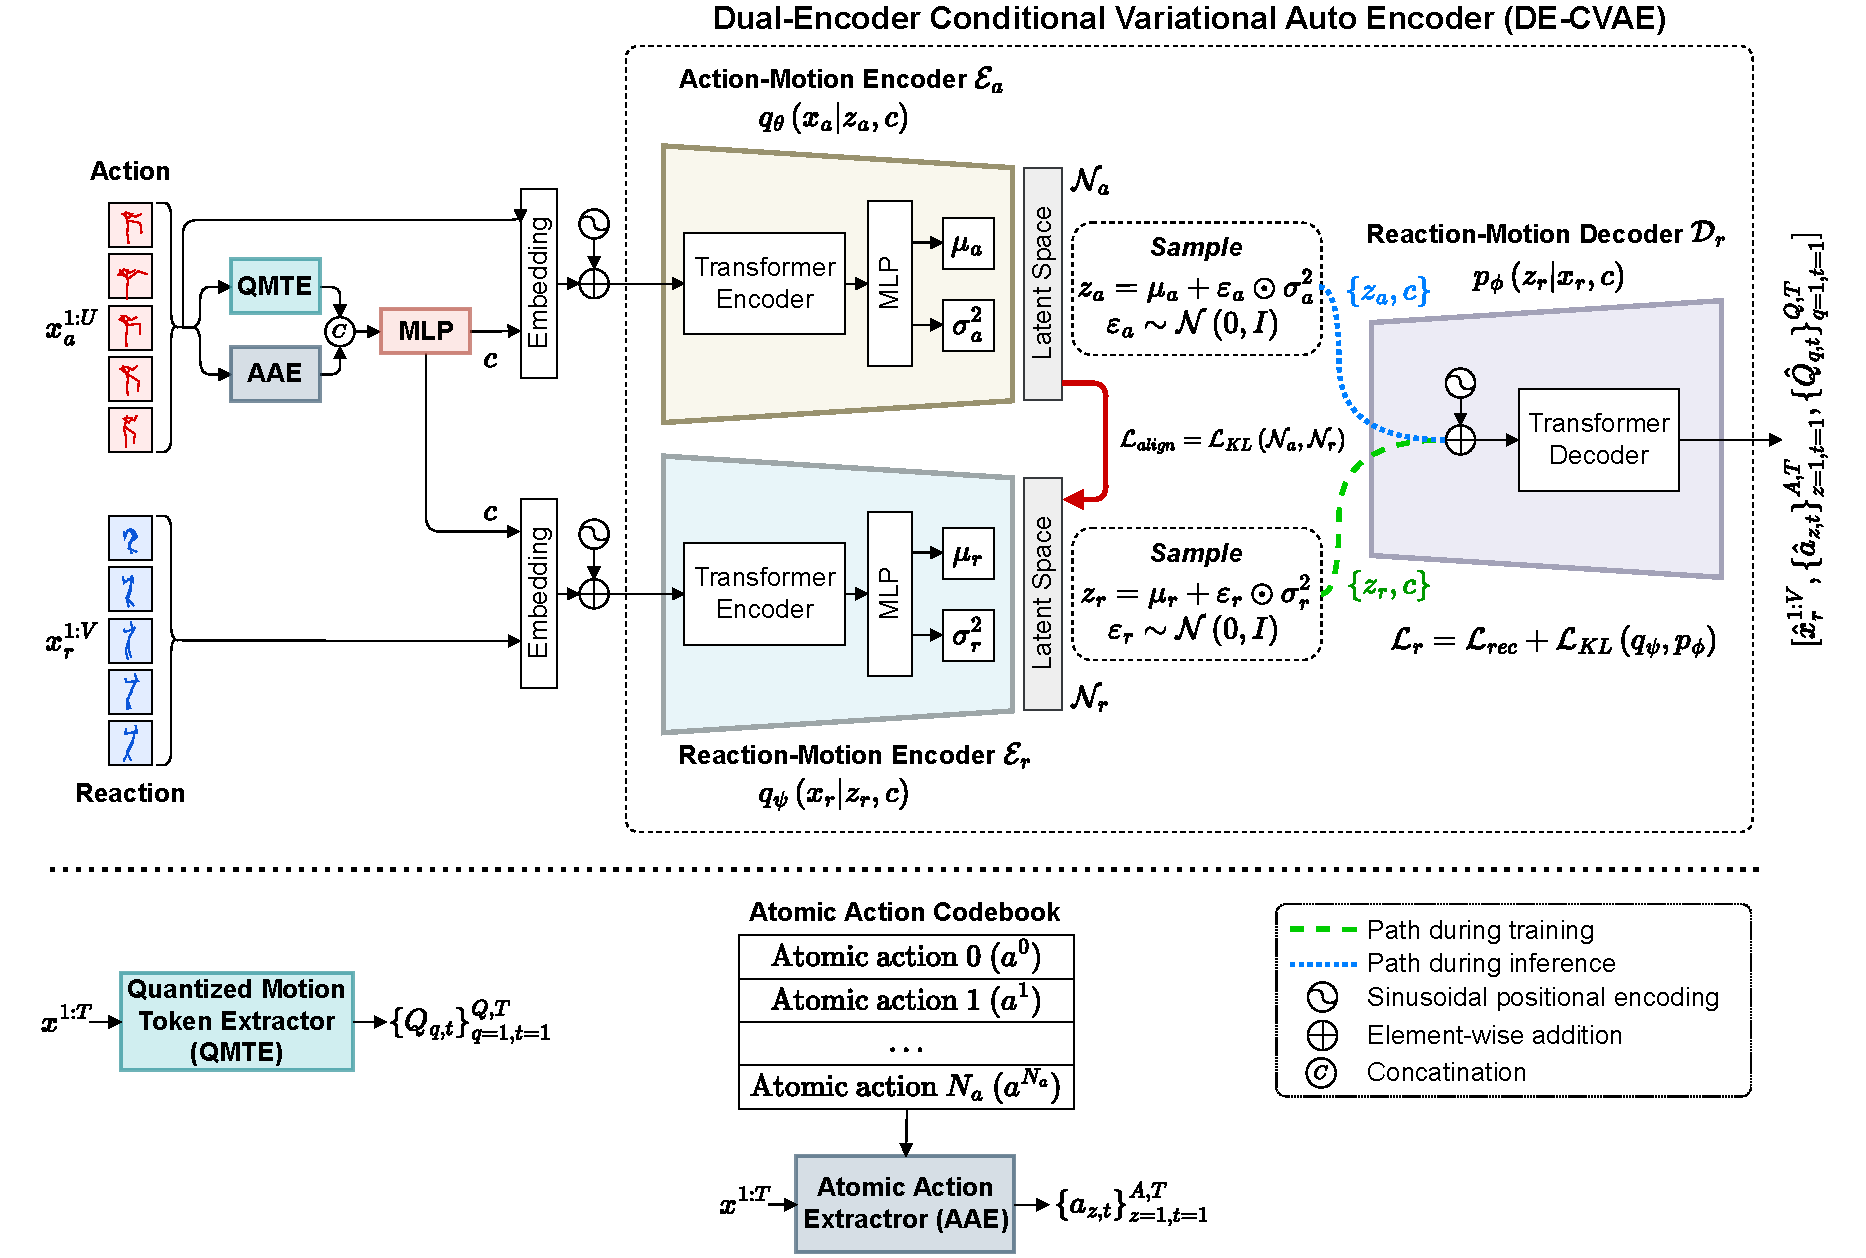
\includegraphics[width=1\textwidth]{figures/chapter4/fig_overview}
	\caption{Overview of the proposed model (left) DE-CVAE network with two encoders and a decoder. QMTs and atomic action vectors are extracted from action-motion using QMTE and AAE modules, respectively (right) QMTE module, AAE module, and atomic action codebook.}
	\label{fig_overview}
\end{figure*}


\section{Related Work}
\subsection{Human Motion Generation}
The human motion generation task aims to produce realistic motion sequences for individuals or interactions involving humans...


\begin{sidewaysfigure}	
	\centering
	\includegraphics[width=0.8\textwidth]{figures/chapter4/fig_qmt}
	\caption{(Top left) Motion sequence (top middle) orientational and positional quantizations (top right) extracted quantized motion tokens (bottom) visual representations for QPT, QPRPT, QPDT, QLAT, QLOT, and QJVT.}
	\label{fig_qmt}
\end{sidewaysfigure}

\section{Method}
\subsection{Problem Formulation}
The human reaction-motion generation task aims to accurately generate the 3D skeleton-based motion of a character, given the action-motion sequence of another character. In the training phase, the input comprises action and reaction motion pairs $ \left\lbrace \left( x_a^{1:U},x_r^{1:V}\right) \right\rbrace  $, where $ x_a^{1:U} $ and $ x_r^{1:V} $ are the action and corresponding reaction-motion sequences, respectively. The motion sequence $ x^{1:T}=\left[ S_1,\dots ,S_T\right]  $ is represented as the human skeleton sequence defined for each discrete time interval $t \in \left\lbrace 1,\dots,T\right\rbrace  $, where $ S_t \in \mathbb{R}^{J \times 3} $ is the human skeleton configuration at any given time $ t $ with $ J=15 $ 3D joint keypoints. Conversely, during the inference phase, our learned model can be expressed as a motion-motion translation function $ G: x_a^{1:U} \rightarrow x_r^{1:V} $.

\subsection{Overview}
The overall pipeline of the proposed method is shown in Fig. \ref{fig_overview}. The method uses an action-motion sequence $ x_a^{1:U}$ and extracts quantized motion tokens and atomic action vectors to generate the conditional signal. The two encoders and a decoder use this conditional signal as a bias to disentangle and regularize the motion spaces. This results in a improved the action-reaction mapping. The reaction-motion encoder encodes ...


\begin{equation}
	\label{eq1}
	{QPT}_t^{(j,\dagger)} = \left\langle {\frac{ s_t^j - s_t^0}{{q_l^p}} }, \frac{{r_t^\dagger}}{{q_l^p}} \right\rangle  - \left\langle \frac{{s_{t-1}^j - s_{t-1}^0}}{{q_l^p}}, \frac{{r_{t-1}^\dagger}}{{q_l^p}} \right\rangle
\end{equation}





\section{Implementation Details}
\label{implementation}
The model was implemented using the open-source PyTorch library. Network weights were initialized randomly and optimized using the Adam optimizer employing a mini-batch size of 32 for 45K epochs. The initial learning rate was set to $ \alpha=10^{-5} $ and decayed gradually with the Step LR scheduler with a step size of 8 and decay rate ...


\section{Experiments}
\label{exp_res}

\subsection{Datasets}
\label{datasets}

\noindent
\textbf{SBU Kinect Interaction Dataset (SBU) \cite{sbu_dataset}} features a skeleton-based two-person interaction dataset collected from the actions of seven individuals organized in 21 pairs of two-actor sets...

\noindent
\textbf{Kinect-based 3D Human Interaction Dataset (K3HI)\cite{k3hi_dataset}} offers a comprehensive repository of rich ...



\begin{sidewaysfigure}	
	\centering
	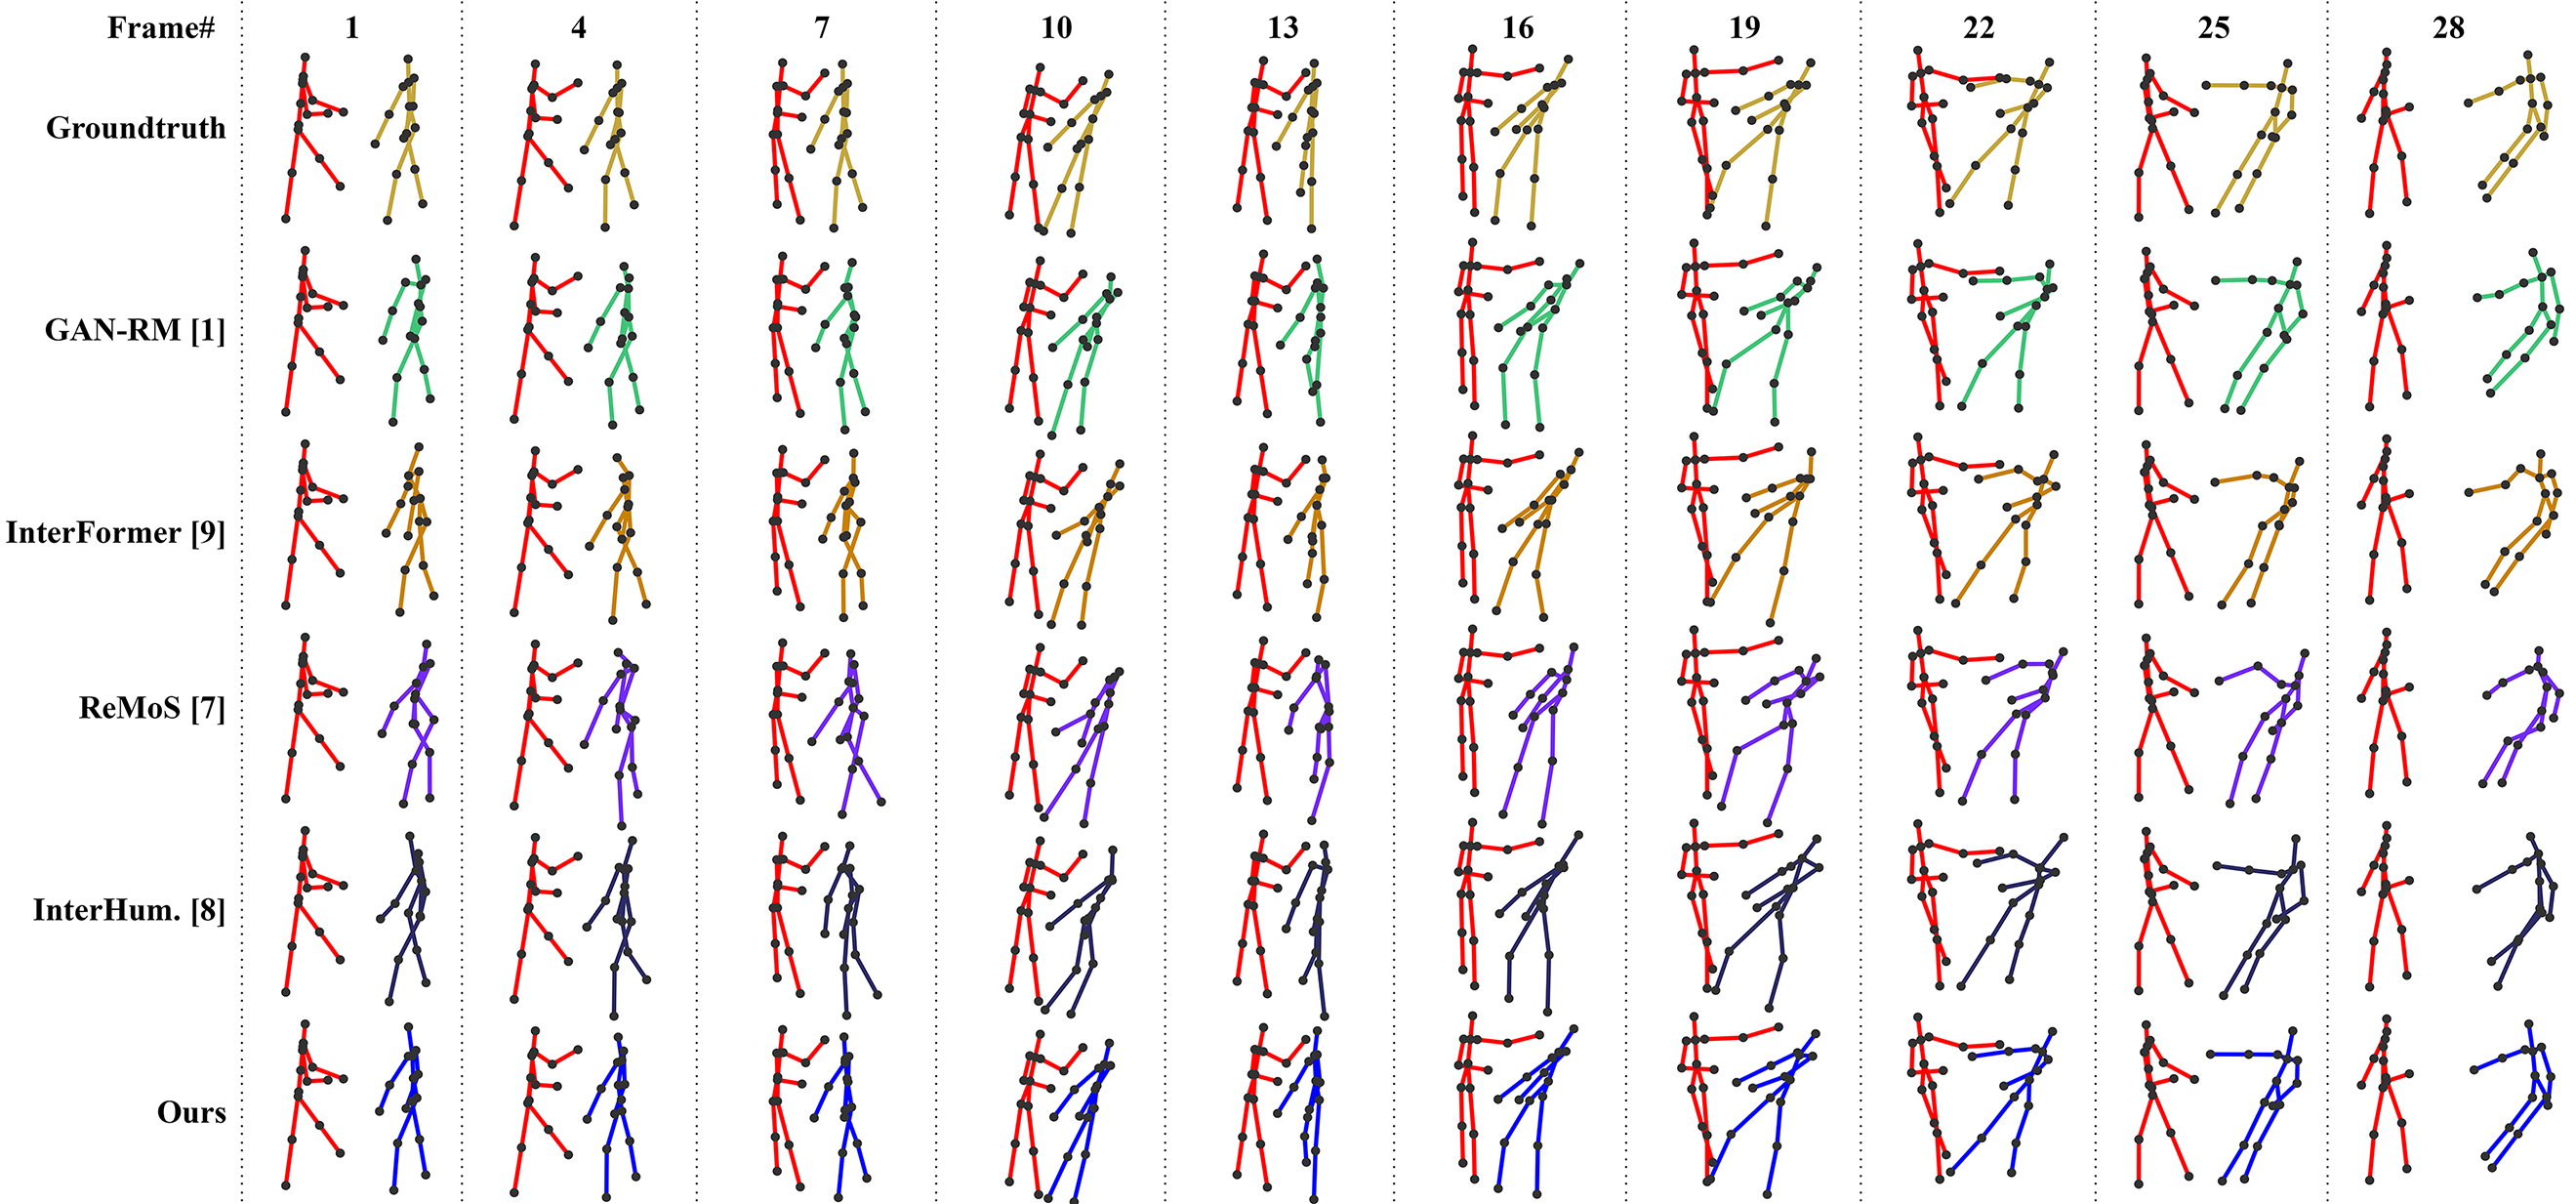
\includegraphics[width=0.9\textwidth]{figures/chapter4/fig_results_sbu}
	\caption{Visualization of motion generation on SBU dataset for punching class. Skeletons in red represent acting character, while the other colors correspond to the reacting character in various methods. (top to bottom) represent motion sequences for groundtruth, generated by methods \cite{gan-reaction-motion}, \cite{interaction_transformer}, \cite{remos}, \cite{interaction-humanoid}, and our results, respectively. (left to right) selective frames during temporal transition.}
	\label{fig_results_sbu}
\end{sidewaysfigure}



\subsection{Evaluation Metrics}
\label{evaluation}

Due to the inherent nature of reaction-motion generation, it is a one-to-many mapping problem...

\noindent
\textbf{The Fr'echet Motion Distance (FMD)} is specifically designed to measure the distance between ground truth and generated data distribution...



\subsection{State-of-the-Art Comparisons}
\label{sota}

\noindent
\textbf{Quantitative Evaluation.} We conducted a comprehensive evaluation of the proposed method by comparing the FMD and diversity evaluation scores on the SBU, DuetDance, and K3HI datasets, as summarized in Table. \ref{table_sota_fmd_div}...






\begin{sidewaystable}
	\centering
	\caption{(Left) Classification accuracy for each class in the SBU, Duetance, and K3HI datasets, comparing our method with groundtruth and exiting approaches (\cite{gan-reaction-motion}, \cite{remos}, \cite{interaction-humanoid}, \cite{interaction_transformer}, \cite{intergen}, and \cite{social-robot}) (right) user perception study, comparing our methods with groundtruth and existing approaches (\cite{interaction_transformer} and \cite{gan-reaction-motion}) across the same datasets. $"\uparrow"$: indicates higher is better. \textbf{Bold} specifies the best results.}
	\label{table_sota_classification_user}
	\renewcommand{\arraystretch}{1.0}
		\begin{tabular*}{1.0\textwidth}{@{\extracolsep{\fill}}l|cccccccc|cccc}	
			\toprule			
			\multirow{2}{*}{Method} &
			GT  &
			GAN-RM  &
			ReMoS  &
			InterHum.  &
			InterFor.  &
			InterGen  &
			Social Rob. &
			Ours &
			GT &
			InterFor. &
			GAN-RM &
			Ours \\ 
			
			&
			&
			\cite{gan-reaction-motion} &
			\cite{remos} &
			\cite{interaction-humanoid} &
			\cite{interaction_transformer} &
			\cite{intergen} &
			\cite{social-robot} &
			&
			&
			\cite{interaction_transformer} &
			\cite{gan-reaction-motion} &
			\\ \hline
			
			\multicolumn{9}{c}{Classification Accuracy $(\uparrow)$} &
			\multicolumn{4}{c}{User Preference $(\uparrow)$} \\ 
			\midrule
			
			\multicolumn{13}{c}{SBU Kinect Interact} \\ 
			\midrule
			
			
			
			
			Walking &89&75&63&60&76&53&44&\textbf{85}&95\%&77\%&80\%&\textbf{89\%}\\
			Kicking &100&\textbf{94}&79&68&82&75&77&93&92\%&\textbf{85\%}&78\%&81\%\\
			Pushing &94&75&71&70&83&68&71&\textbf{91}&88\%&77\%&\textbf{78\%}&73\%\\
			Shaking Hands &97&\textbf{91}&72&67&82&73&71&87&86\%&70\%&73\%&\textbf{82\%}\\
			Exchanging &95&\textbf{89}&69&82&72&66&67&88&89\%&78\%&\textbf{88\%}&76\%\\
			Punching &100&90&78&75&88&78&76&\textbf{93}&93\%&72\%&75\%&\textbf{90\%}\\
			Average &95.83&85.67&72&70.33&80.5&68.83&67.67&\textbf{89.5}&90.5\%&76.5\%&78.67\%&\textbf{81.83\%}\\ 
			\midrule
			
			\multicolumn{13}{c}{DuetDance} \\ 
			\midrule
			
			
			
			
			Cha-Cha &94&80&73&68&74&69&53&\textbf{87}&88\%&74\%&76\%&\textbf{82\%}\\
			Jive &95&86&70&71&81&69&73&\textbf{93}&79\%&62\%&\textbf{76\%}&74\%\\
			Rumba &92&78&66&67&78&67&64&\textbf{85}&78\%&68\%&66\%&\textbf{74\%}\\
			Salsa &97&\textbf{93}&75&73&78&70&71&92&84\%&66\%&75\%&\textbf{79\%}\\
			Samba &96&77&74&69&\textbf{89}&71&60&82&85\%&75\%&70\%&\textbf{83\%}\\
			Average &94.8&82.8&71.6&69.6&80&69.2&64.2&\textbf{87.8}&82.8\%&69\%&72.6\%&\textbf{78.4\%}\\ 
			\midrule
			
			\multicolumn{13}{c}{K3HI} \\ 
			\midrule
			
			
			Approaching &98&84&72&78&78&72&65&\textbf{97}&88\%&74\%&78\%&\textbf{81\%}\\
			Departing &93&90&68&82&66&69&68&\textbf{93}&84\%&72\%&76\%&\textbf{80\%}\\
			Kicking &100&82&72&93&76&75&70&\textbf{94}&89\%&\textbf{86\%}&76\%&85\%\\
			Pushing &100&\textbf{96}&77&84&76&72&74&95&89\%&78\%&74\%&\textbf{85\%}\\
			Shaking &96&\textbf{94}&68&75&75&71&71&90&87\%&76\%&78\%&\textbf{84\%}\\
			Exchanging &93&77&72&84&70&69&48&\textbf{93}&90\%&78\%&\textbf{88\%}&86\%\\
			Punching &100&89&75&90&82&71&74&\textbf{94}&90\%&72\%&80\%&\textbf{89\%}\\
			Pointing &94&81&68&87&66&70&67&\textbf{89}&86\%&73\%&\textbf{86\%}&84\%\\
			Average &96.75&86.62&71.5&84.12&73.62&71.125&67.12&\textbf{93.12}&87.87\%&76.12\%&79.5\%&\textbf{84.25\%}\\ 
			\midrule
			
	\end{tabular*}
\end{sidewaystable}


\noindent
\textbf{Qualitative Evaluation.} We performed a qualitative evaluation by visually comparing the motion sequences generated by the proposed method with the groundtruth and various SOTA methods. Fig. \ref{fig_results_sbu}, \ref{fig_results_k3hi}, and \ref{fig_results_duetdance} show the qualitative comparisons of the test samples from ...


\noindent
\textbf{Perceptual User Study.} Relying solely on quantitative evaluation and self-performed qualitative analysis is insufficient due to the intricacies of the problem at hand. For a more comprehensive visual assessment of motion quality, ...


\subsection{Ablation Study}
\label{ablation}
To assess the effectiveness of the proposed modules in our network, we performed an ablation study on the SBU dataset, focusing on the diversity and FMD metrics. We set up four versions of our model and tested them with different ... 

\section{Conclusion}
\label{conclusion}
In this paper, we introduce a novel DE-CVAE network featuring two encoders designed for the task of human reaction motion generation... 


\section{Future Work}
\label{future}
Despite significant improvements in the generation task, our approach faces three major challenges. (1) As the interactions...




\backmatter

% Conclusion
%%
% The BIThesis Template for Graduate Thesis
%
% Copyright 2020-2023 Yang Yating, BITNP
%
% This work may be distributed and/or modified under the
% conditions of the LaTeX Project Public License, either version 1.3
% of this license or (at your option) any later version.
% The latest version of this license is in
%   http://www.latex-project.org/lppl.txt
% and version 1.3 or later is part of all distributions of LaTeX
% version 2005/12/01 or later.
%
% This work has the LPPL maintenance status `maintained'.
%
% The Current Maintainer of this work is Feng Kaiyu.

\begin{conclusion}

In this study, we address the long-standing challenge of bridging raw human motion and action semantics via fuzzy qualitative kinematics. By combining fuzzy logic and qualitative kinematic reasoning, we proposed a novel ...

\end{conclusion}


% References
%%
% The BIThesis Template for Graduate Thesis
%
% Copyright 2020-2023 Yang Yating, BITNP
%
% This work may be distributed and/or modified under the
% conditions of the LaTeX Project Public License, either version 1.3
% of this license or (at your option) any later version.
% The latest version of this license is in
%   http://www.latex-project.org/lppl.txt
% and version 1.3 or later is part of all distributions of LaTeX
% version 2005/12/01 or later.
%
% This work has the LPPL maintenance status `maintained'.
%
% The Current Maintainer of this work is Feng Kaiyu.

%
% 如无特殊需要,本页面无需更改


\begin{bibprint}
  \printbibliography[heading=none,notcategory=main,resetnumbers=true]
\end{bibprint}


% Appendices
%%
% The BIThesis Template for Graduate Thesis
%
% Copyright 2020-2023 Yang Yating, BITNP
%
% This work may be distributed and/or modified under the
% conditions of the LaTeX Project Public License, either version 1.3
% of this license or (at your option) any later version.
% The latest version of this license is in
%   http://www.latex-project.org/lppl.txt
% and version 1.3 or later is part of all distributions of LaTeX
% version 2005/12/01 or later.
%
% This work has the LPPL maintenance status `maintained'.
%
% The Current Maintainer of this work is Feng Kaiyu.

\begin{appendices}
  \chapter{SMPL Parameter Settings}
  This is optional ...

\end{appendices}


% Personal achievements
%%
% The BIThesis Template for Graduate Thesis
%
% Copyright 2020-2023 Yang Yating, BITNP
%
% This work may be distributed and/or modified under the
% conditions of the LaTeX Project Public License, either version 1.3
% of this license or (at your option) any later version.
% The latest version of this license is in
%   http://www.latex-project.org/lppl.txt
% and version 1.3 or later is part of all distributions of LaTeX
% version 2005/12/01 or later.
%
% This work has the LPPL maintenance status `maintained'.
%
% The Current Maintainer of this work is Feng Kaiyu.

% 1. 在 `./reference/pub.bib` 中添加数据。
% 2. 在下方 `\addpubs` 添加该文献(参考下方示例)。

% **注意:如果发现渲染出来的文献编号不正确,请使用 `latexmk -c` 清除缓存后重新编译。**

\begin{publications}

  \addpubs{pub1, pub2, pub3, pub4, patent:1, patent:2, patent:3, patent:4}

  % Mainly for master’s students
%  \printbibliography[heading=none,category=mypub,resetnumbers=true]

  % If you want to divide it into multiple lists, you can use the following command.
  % Mainly for doctoral students.
  \pubsection{Articles}
  
  \printbibliography[heading=none,type=article,category=mypub,resetnumbers=true]{}
  %
  % \pubsection{Books}
  %
  % \printbibliography[heading=none,type=book,category=mypub,resetnumbers=true,notkeyword=dummy]{}
  %
  \pubsection{Patents}

  \printbibliography[heading=none,type=book,category=mypub,resetnumbers=true]{}

\end{publications}



% Acknowledgments
%%
% The BIThesis Template for Graduate Thesis
%
% Copyright 2020-2023 Yang Yating, BITNP
%
% This work may be distributed and/or modified under the
% conditions of the LaTeX Project Public License, either version 1.3
% of this license or (at your option) any later version.
% The latest version of this license is in
%   http://www.latex-project.org/lppl.txt
% and version 1.3 or later is part of all distributions of LaTeX
% version 2005/12/01 or later.
%
% This work has the LPPL maintenance status `maintained'.
%
% The Current Maintainer of this work is Feng Kaiyu.

\begin{acknowledgements}


First and foremost, ...



\end{acknowledgements}


% Personal profile (only required for doctoral students)
%%
% The BIThesis Template for Graduate Thesis
%
% Copyright 2020-2023 Yang Yating, BITNP
%
% This work may be distributed and/or modified under the
% conditions of the LaTeX Project Public License, either version 1.3
% of this license or (at your option) any later version.
% The latest version of this license is in
%   http://www.latex-project.org/lppl.txt
% and version 1.3 or later is part of all distributions of LaTeX
% version 2005/12/01 or later.
%
% This work has the LPPL maintenance status `maintained'.
%
% The Current Maintainer of this work is Feng Kaiyu.

\begin{resume}

The author ...

\end{resume}



\end{document}
